\section{La page des terrains}

Vous êtes l'heureux propriétaire d'un terrain de tennis ? C'est par ici !

\subsection{Gérer ses terrains}

\textbf{Si vous n'avez pas de terrains enregistrés}, vous pouvez en ajouter un
en cliquant sur \textit{Enregistrer un nouveau terrain}. Vous serez amené à
compléter un formulaire nous permettant de savoir les disponibilités de votre
terrain ainsi que les informations d'accès utiles à nos joueurs.

\begin{figure}[H]
\centering
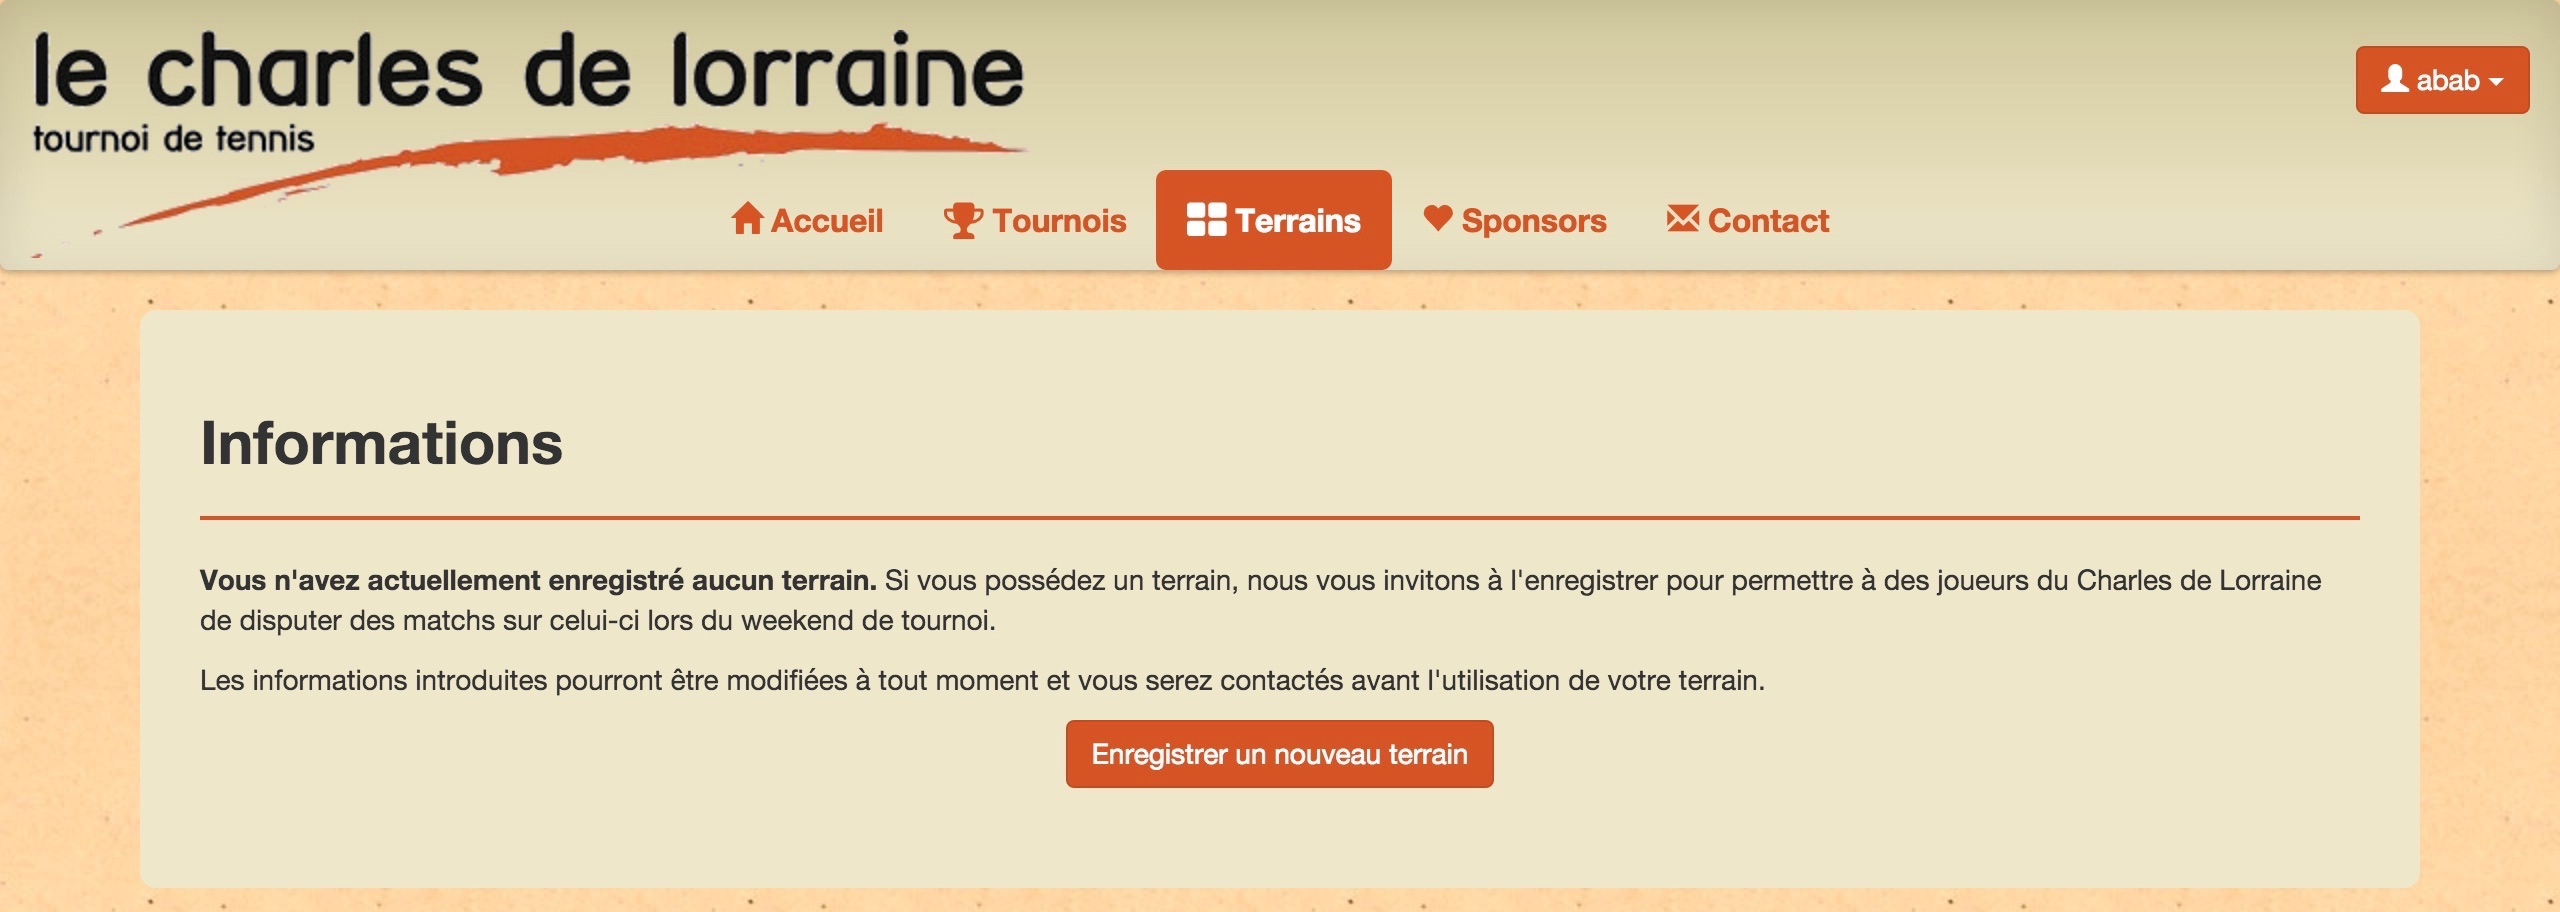
\includegraphics[scale=0.15]{page-terrains/page-terrains-sans.jpg}
\caption{Page des terrains - aucun terrain enregistré}
\end{figure}

\textbf{Si vous avez déjà un terrain enregistré} :

\begin{itemize}
    \item Vous pouvez accéder à ses informations et les modifier en cliquant
    sur le résumé du terrain.
    \item Vous pouvez supprimer votre terrain si vous ne souhaitez plus que
    le Charles de Lorraine puisse l'utiliser. Nous serions ravis si vous
    pouviez au préalable nous en informer via notre formulaire de contact pour
    assurer la bonne gestion du tournoi ;
    % TODO
    \todo[inline]{Ajouter une référence vers le formulaire de contact}
    \item Vous aurez accès aux informations d'utilisation de votre terrain pour
    savoir si votre terrain sera utilisé pour le tournoi. Ces informations
    sont mises à jour lorsque l'équipe aura assigné les joueurs dans les
    tournois ;
    \item Vous pouvez ajouter un terrain supplémentaire en cliquant sur le
    bouton \textit{Enregistrer un nouveau terrain} et vous serez ainsi dirigé
    vers un formulaire identique à celui complété pour le premier terrain.
\end{itemize}

\begin{figure}[H]
\centering
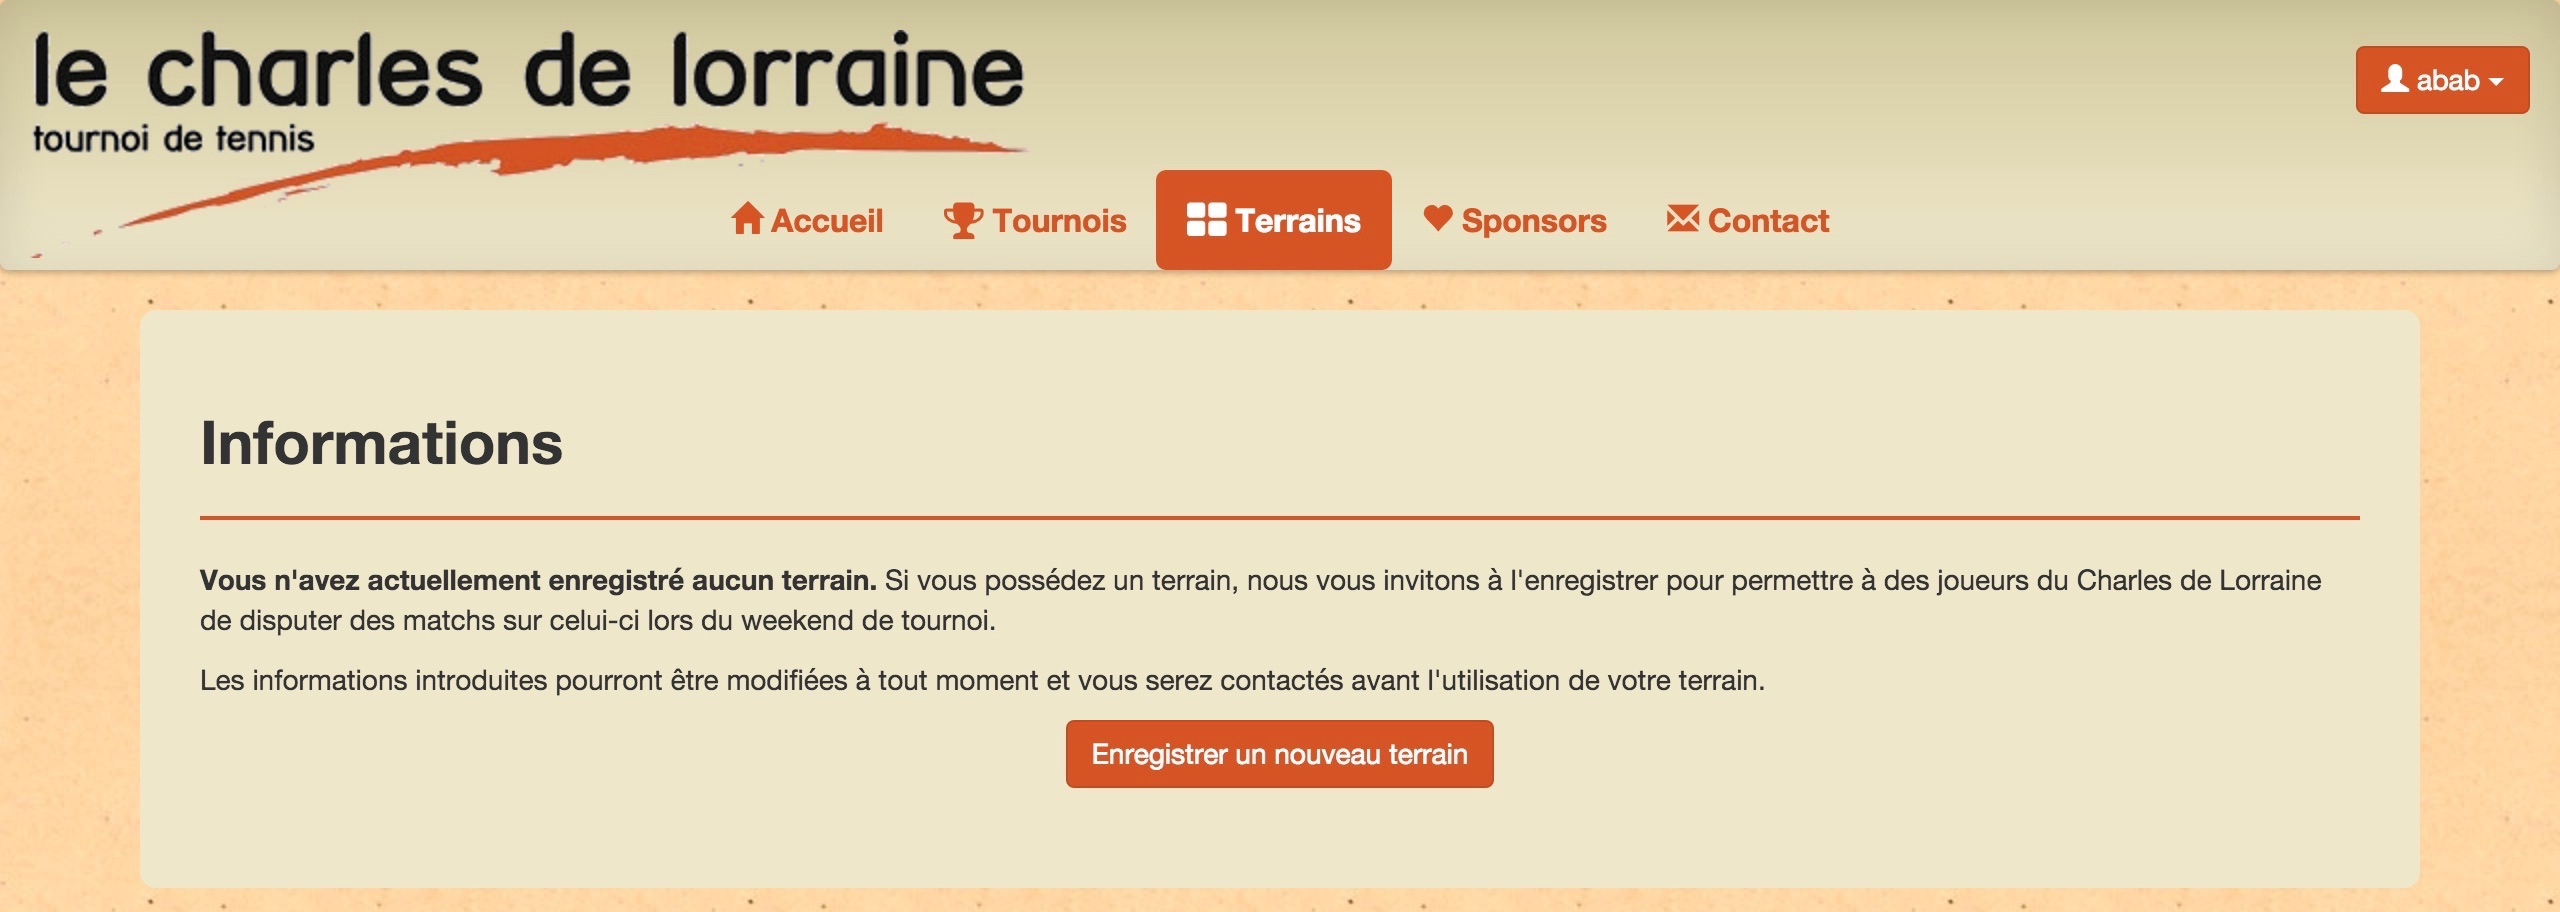
\includegraphics[scale=0.15]{page-terrains/page-terrains-sans.jpg}
\caption{Page des terrains - terrains enregistrés}
\end{figure}
